\documentclass[twocolumn,10pt]{article}

\usepackage[utf8]{inputenc}
\usepackage{amsmath, amssymb, amsfonts, amsthm}
\usepackage{upgreek}
\usepackage{amsthm}
\usepackage{fullpage}
\usepackage{graphicx}
\usepackage{cancel}
\usepackage{subfigure}
\usepackage{mathrsfs}
\usepackage{enumerate}
%\usepackage{outlines}
\usepackage[font={sf,it}, labelfont={sf,bf}, labelsep=space, belowskip=5pt]{caption}
\usepackage{hyperref}
% \usepackage{minted}

\usepackage{float}
% \floatplacement{figure}{H}

\usepackage{fancyhdr}
\usepackage[title]{appendix}
\usepackage{siunitx}

\DeclareMathOperator{\tr}{tr}
\DeclareMathOperator{\sgn}{sgn}
\DeclareMathOperator{\sinc}{sinc}
\DeclareMathOperator{\rref}{rref}
\DeclareMathOperator{\cof}{cof}

\providecommand{\abs}[1]{\lvert#1\rvert}
\providecommand{\norm}[1]{\lVert#1\rVert}
\providecommand{\dx}{\, \mathrm{d}x}
\providecommand{\dA}{\, \mathrm{d}A}
% \providecommand{\vint}[2]{\int_{#1} \! #2 \, \mathrm{d}x}
% \providecommand{\sint}[2]{\int_{\partial #1} \! #2 \, \mathrm{d}A}
\renewcommand{\div}{\nabla \cdot}
\providecommand{\e}{\epsilon}
\providecommand{\shape}{\Omega(p)}
\providecommand{\boundary}{\partial \shape}
\providecommand{\vint}[1]{\int_{\shape} \! #1 \, \mathrm{d}x}
\providecommand{\sint}[1]{\int_{\boundary} \! #1 \, \mathrm{d}A}
\providecommand{\pder}[2]{\frac{\partial #1}{\partial #2}}
\providecommand{\tder}[2]{\frac{\mathrm{d} #1}{\mathrm{d} #2}}
\providecommand{\evalat}[2]{\left.#1\right|_{#2}}
\newcommand{\defeq}{\vcentcolon=}
\newtheorem{lemma}{Lemma}
\newcommand\numberthis{\addtocounter{equation}{1}\tag{\theequation}}

\makeatletter
\usepackage{mathtools}
\newcases{mycases}{\quad}{%
  \hfil$\m@th\displaystyle{##}$}{$\m@th\displaystyle{##}$\hfil}{\lbrace}{.}
\makeatother
\DeclarePairedDelimiter\ceil{\lceil}{\rceil}
\DeclarePairedDelimiter\floor{\lfloor}{\rfloor}

\newenvironment{amatrix}[1]{%
  \left[\begin{array}{@{}*{#1}{c}|c@{}}
}{%
  \end{array}\right]
}

%% + Abtin
\usepackage{fullpage}
\usepackage[usenames,dvipsnames]{color}
\usepackage{paralist}
\usepackage{prettyref}
\newrefformat{sec}{Section~\ref{#1}}
\newrefformat{tbl}{Table~\ref{#1}}
\newrefformat{fig}{Fig.~\ref{#1}}
\newrefformat{chp}{Chapter~\ref{#1}}
\newrefformat{eqn}{Eq.~\eqref{#1}}
\newrefformat{set}{Eq.~Set~\eqref{#1}}
\newrefformat{alg}{Algorithm~\ref{#1}}
\newrefformat{apx}{Appendix~\ref{#1}}
\newcommand\pr[1]{\prettyref{#1}}

\newcommand\todo[1]{\textcolor{magenta}{\bf [TODO: #1]}}
\renewcommand\vec[1]{\ensuremath{\mathbf #1}}
\def\x{\vec{x}}
\def\y{\vec{y}}
\def\u{\vec{u}}
\def\ue{\vec{u}^\e}
\def\strain{\varepsilon}


\begin{document}
\section{Periodic Homogenization\label{sec:homogen}}
Considering a heterogeneous object $\Omega^\e$ with periodic
microstructures of size $\e$, as shown schematically in
\pr{fig:periodic}, our goal is to find the homogenized elasticity
tensor $C^H$ as the effective elasticity tensor of the object (defined
more rigorously below). Parameter $\e$ determines the size of cell $Y$
relative to the domain $\Omega^\e$ and permits us to perform
asymptotic analysis.
\begin{figure}[!hbt]
    \centering
    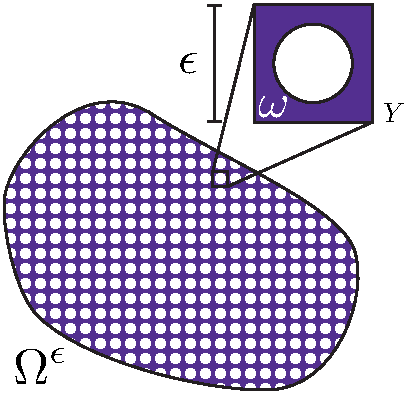
\includegraphics[width=.28\textwidth]{Images/periodic.pdf}
    \caption{(Schematic) Periodic tiling of a domain $\Omega$ with
      base cell $Y$ having geometry $\omega$ and length scale $\e$.}
    \label{fig:periodic}
\end{figure}

The elastic response of an object under external load $\vec{f}$ is
governed by linear elasticity equation
\begin{equation}
  \label{eqn:elastostatic}
  -\nabla \cdot [C : \strain(\ue)] = \vec{f} \text{ in }\Omega^\e,
\end{equation}
complemented by appropriate boundary conditions. Considering a
sequence of problems indexed by $\e$ and letting $\vec{u}$ denote the
limit of $\ue$ as $\e\to 0$, the homogenized elasticity tensor $C^H$
is defined as the tensor that satisfies
\begin{equation}
    \label{eqn:homogenElasto}
  -\nabla \cdot [C^H : \strain(\u)] = \vec{f} \text{ in }\Omega,
\end{equation}
with same boundary conditions. Vectors $\u$ and $\ue$ denotes the
displacement, $C$ is the local elasticity tensor, and $\strain(\u)
\coloneqq \frac{1}{2}(\nabla \u + (\nabla \u)^T )$ is the Cauchy
strain tensor (defined similarly for $\ue$).

Here we outline the periodic homogenization method using the two-scale
asymptotic expansion method with minimal mathematical justification
and refer the reader to \cite{allaire2002shape,
  allaire1992homogenization, defranceschi1993} for more detail and
rigorous justification. The mathematical difficulty of a framework
that takes \pr{eqn:elastostatic} to \pr{eqn:homogenElasto} is to
define the proper notion of convergence as $\e\to 0$. The two-scale
method is based on the ansatz that for small $\e$, the family of
solutions $\ue$, parameterized by $\e$, can be written as
\begin{equation}
  \label{eqn:AsymSeries}
  \ue(\x) = \sum_{p = 0}^{\infty} \e^p \u_p\left(\x, \frac{\x}{\e}\right).
\end{equation}
Each term $\u_p(\x,\y)$ is a $Y$-periodic function of $\y$.

The method of two-scale asymptotic expansions is a heuristic method
and the above assumption is usually not correct after the first two
terms; nonetheless, it is possible to rigorously justify the
homogenization process and the convergence of the sequence $\ue$ to
the solution $\u$ (usually by means of the so-called energy method)
\cite{allaire2002shape, allaire1992homogenization}.

As implied by \pr{eqn:homogenElasto} and \pr{eqn:AsymSeries}, the
first term of the series $\u_0$ is identified with the solution of the
homogenized equation $\u$. Knowing $\u$ for proper choices of
$\vec{f}$, the effective elasticity tensor $C^H$ can be computed. Note
that the homogenized tensor $C^H$ is almost never a spatial average of
$C$.

To facilitate the analysis, let \x\ denote the macroscopic variable
and define $\y\coloneqq \x/\e$ as the microscopic variable. For ${\y}
\in Y$, the local elasticity tensor is given as
\begin{equation}
  \label{eqn:microC}
  C(\y) = \begin{cases} C^\text{base} & \text{if } \y
    \in \omega, \\ 0 & \text{ otherwise,} \end{cases}
\end{equation}
where $C^\text{base}$ is the known material property and is extended
throughout $\Omega$ by $Y$-periodicity.

Let $\vec{e}^{kl} \coloneqq \frac{1}{2} \left(\vec{e}_k \otimes
\vec{e}_l + \vec{e}_l \otimes \vec{e}_k \right)$ denote the canonical
basis for symmetric rank 2 tensors and define $\vec{w}^{kl}$ as the
microscopic displacements response for $\vec{e}^{kl}$ satisfying
\begin{subequations}
  \label{set:cell}
  \begin{gather}
    \nabla \cdot (C^\text{base} : \strain({\bf w}^{kl})) = 0 \text{ in } \omega, \\
    [C^\text{base} : \strain({\bf w}^{kl})]\hat{\vec{n}}  =  - [C^\text{base} : \vec{e}^{kl}]\hat{\vec{n}} \text{ on } \partial \omega \backslash \partial Y, \\
    {\bf w}^{kl}({\y})\ Y\text{-periodic}, \\
    \int_\omega \! {\bf w}^{kl}({\y})  \, \mathrm{d} {\y} =  {\bf 0},
  \end{gather}
\end{subequations}
where the last constraint is to pin down the translational degrees of
freedom; since we only care about strain $\strain(\vec{w}^{kl})$.  We
refer to \pr{set:cell} as the cell problem.

Knowing $\vec{w}^{kl}$, the effective elasticity tensor is expressed
as an integral over the cell $Y$
\begin{equation}
  \label{eqn:effective}
  C^H_{ijkl} = \frac{1}{|Y|} \int_\omega C_{ijpq}^\text{base}[\strain(\vec{w}^{kl})]_{pq} + C_{ijkl}^\text{base} \, \mathrm{d} \y.
\end{equation}
See \pr{apx:asymptotic} for the connection between \pr{set:cell} and
\pr{eqn:effective} and more detail on their derivation.

It is worth noting that $C^H$ does not depend on the choice of domain
$\Omega$, force term $\vec{f}$, or boundary condition on $\partial
\Omega$.

For each cell shape, \pr{set:cell} needs to be solved numerically for
the six---instead of nine because of the symmetry in canonical basis
$(\vec{e}^{kl} = \vec{e}^{lk})$---cell problems to compute
$\vec{w}^{kl}\;(k,l=1,2,3)$, which are in turn used to evaluate
\pr{eqn:effective}.

\subsection{FEM Implementation}
The cell problems (\pr{set:cell}) are solved numerically by FEM
discretization of a single base cell. The volume integral
(\pr{eqn:effective}) is computed on the same grid.

Given the wire network of the microstructure, defining its topology
\todo{internal ref}, a volume mesh is generated following the STRUT
algorithm given in \cite{hart2008sculptural} involving the following
steps:\begin{inparaenum}[(i)]
\item A polygon is created around both ends of each segment.
\item For each vertex, the convex hull of the nearby polygons and the
  vertex is constructed and the polygons themselves are removed from
  the hull.
\item For each edge, the convex hull of its two polygons is
  constructed, and again the two polygons are removed from the hull.
\end{inparaenum}
The volume mesh is then used to generated the tetrahedron elements for
the FEM computation.

The linear elasticity solver needs to support periodic boundary
conditions, which requires the tet-based volume mesh to have identical
tessellation on opposite periodic cell faces. Periodic boundary
conditions are implemented by direct elimination of variables. Direct
elimination is performed by assigning all mesh or grid nodes in each
connected component of the identified vertex graph the same degrees of
freedom. For example, the cell's corner nodes---if they exist---appear
as the graph's only component of size 8 and all get the same $x$, $y$,
and $z$ displacement degrees of freedom. Edge nodes will appear in a
component of size 4.

To simplify operations such as rank 4 tensor inversion and double
contractions, we use a symmetric tensor flattening approach to turn
rank 4 tensors into matrices and rank 2 tensors into vectors. We end
up storing the elasticity tensor as a symmetric $6\times 6$ matrix
with 21 coefficients. \todo{give ref}.

\appendix
\section{Asymptotic Analysis for Periodic Homogenization\label{apx:asymptotic}}
As outlined in \pr{sec:homogen}, the homogenization process proceeds
by considering the solution of \pr{eqn:elastostatic}, the displacement
$\ue$, as $\e\to 0$. One approach in taking this limit is through
two-scale asymptotic expansions \cite{allaire2002shape}. Further
detail can be found in
\cite{allaire2002shape,allaire1992homogenization}, here we outline
major steps in the derivation of $C^H$.

\subsection{Two-scale Analysis}
As mentioned in \pr{sec:homogen}, the two-scale method is based on the
ansatz that for small $\e$, the family of solutions $\ue$,
parameterized by $\e$, can be written as
\begin{equation}
  \ue(\x) = \sum_{p = 0}^{\infty} \e^p \u_p\left(\x, \frac{\x}{\e}\right).
\end{equation}
Each function $\u_p$ separates its dependence on $\x$ (i.e. the
smoothly varying, macroscopic part) from its dependence on $\y =
\x/\e$ (the microscopic fluctuations). Plugging the series into
\pr{eqn:elastostatic}, collecting coefficients of $\e^p$ terms, and
identifying each coefficient of $\e^p$ of as an individual equation,
yields a cascade of equations for $\u_p$
\begin{align}
  \e^{-2}&:\; -\nabla_\y \cdot [C(\y) : \strain_\y(\u_0)] = \vec{0} \label{eqn:em2} \\
  \e^{-1}&:\; -\nabla_\y \cdot [C(\y) : (\strain_\y(\u_1) + \strain_\x(\u_0))] - \phantom{x}\notag\\
  &\hspace{.12\linewidth} \nabla_\x \cdot [C(\y) : \strain_\y(\u_0)] =  \vec{0},  \label{eqn:em1} \\
  \e^{0}&:\; -\nabla_\y \cdot [C(\y) : (\strain_\y(\u_2) + \strain_\x(\u_1))] - \phantom{x}\notag\\
  &\hspace{.12\linewidth} \nabla_\x \cdot [C(\y) : (\strain_\y(\u_1)+\strain_\x(\u_0))] =  \vec{f},\label{eqn:em0}
\end{align}
where the subscripts $\x$ or $\y$ imply derivative with respect to
that variable. \pr{eqn:em2} is satisfied by a function independent of
$\y$, $\u_0(\x,\y)\equiv \u(\x)$. Using this, \pr{eqn:em1} implies a
linear relationship between $\strain_\y(\u_1)$ and $\strain_\x(\u)$,
which we can express with a rank 4 tensor $F$ such that
\begin{equation}
  \label{eqn:macro2micro}
  \strain_\y(\u_1) = F:\strain_\x(\u),
\end{equation}
mapping macroscopic strain to microscopic fluctuation strain.

The term for $\e^0$ uniquely defines $\vec{u}_2$ based on $\vec{u}$
and $\vec{u}_1$ if and only if the compatibility condition of the
Fredholm alternative (zero average right hand side) is
satisfied. Integrating the $\e^0$ term, using Divergence theorem and
periodicity of $\vec{u}_1$ and $\vec{u}_2$ we have
\[
  -\nabla_\x \cdot \int_Y C(\y) : [\strain_\y(\u_1) + \strain_\x(\u)] \, \mathrm{d} \y = |Y| {\bf f}.
\]
Using \pr{eqn:macro2micro}
\begin{equation}
  -\nabla_\x \cdot \left[ \left(\frac{1}{|Y|} \int_Y C(\y) : F + C(\y) \, \mathrm{d} {\bf y} \right) : \strain_\x(\u) \right] = \vec{f},
\end{equation}
Comparing this with \pr{eqn:homogenElasto} implies
\begin{equation}
  C^H = \frac{1}{|Y|} \int_Y C(\y) : F + C(\y) \, \mathrm{d} {\y}
\end{equation}

\subsection{Local Microscopic Displacement}
It remains to determine rank 4 tensor $F$ appearing in $C^H$ using
\pr{eqn:em1}. Letting $\vec{e}^{kl}$ to denote canonical basis for
symmetric rank 2 tensors:
\[
\vec{e}^{kl} = \frac{1}{2} \left({\bf e}_k \otimes {\bf e}_l + {\bf
  e}_l \otimes {\bf e}_k \right)
\]
where ${\bf e}_k$ is the $k^\text{th}$ canonical basis. Then the
macroscopic strain can be decomposed as $\strain_{\x}({\bf u}) =
[\strain_{\x}({\bf u})]_{kl}\vec{e}^{kl}$. If Y-periodic ${\bf
  w}^{kl}({\y})$ solves (\ref{eqn:em1}) for $\vec{e}^{kl}$:
\begin{equation}
-\nabla_{\y} \cdot (C(\y): [\strain_\y({\bf w}^{kl}) +
  \vec{e}^{kl}]) = \vec{0}.
\end{equation}
By linearity, $\strain_\y(\u_1) =
[\strain_\x(\u)]_{kl}\strain_\y(\vec{w}^{kl})$, implying
\begin{equation}
F_{pqkl} = [\strain_{\y}({\bf w}^{kl})]_{pq}
\end{equation}
Plugging this into the equation for the homogenized elasticity
coefficients, we get
\begin{equation}
    \label{eqn:Eh}
    C^H_{ijkl}= \frac{1}{|Y|} \int_Y C_{ijpq}({\y}) [\strain_{\y}({\bf
        w}^{kl})]_{pq} + C_{ijkl}({\y}) \, \mathrm{d} {\y}.
\end{equation}
Once we know each ${\bf w}^{kl}$, we can compute the homogenized
elasticity tensor with a simple integration over the base cell. We
find these by solving the 6 cell problems
\begin{subequations}
  \begin{gather}
    -\nabla_{\y} \cdot (C(\y):[\strain_\y(\vec{w}^{kl}) + \vec{e}^{kl}]) = \vec{0} \quad \text{in } Y, \\
    \vec{w}^{kl}(\y)\ Y \text{-periodic}, \\
    \int_\omega \! \vec{w}^{kl}(\y) \, \mathrm{d} {\y} =  \vec{0}.
  \end{gather}
\end{subequations}
One for each canonical basis tensor $\vec{e}^{kl}$. The last
constraint is to fix the remaining transnational degree of freedom;
since we only care about strain $\strain_{\y}({\bf w}^{kl})$, we can
arbitrarily choose to enforce $\vec{0}$ average displacement over the
microstructure geometry.

\bibliographystyle{plain}
\bibliography{references}

\end{document}
